\section{Proposed Random Address Translator (RAT)}

From the analysis in the previous sections, it is prominent that the existence of linear correlation between index Bytes of the state matrix and the location of corresponding accessed block in memory is the primary reason of vulnerability of AES in the first round. Given size of memory block (64 Bytes in most of the cases), any information about the memory access during the encryption process would directly reveal high nibble of the index Bytes. Thus if the size of the key is 128 Bit, pre-knowledge of the high nibbles of the index Bytes would reduce the brute force complexity to $2^{64}$. A machine that can perform 1 quadrillion operations per seconds would take less than 5 seconds to break the rest of the key in brute force attempt.\\

If the correlation can be broken, so that the index Byte will no longer be used directly to locate the desired block of the Lookup table, most of the cache-timing threats will be eliminated. The key concept to the solution is to perform memory access to get the desired content from an arbitrary, unpredictable location. This can be accomplished by introducing a Translator table between the state matrix and the Lookup table.\\

The most common picture that one might perceive in such a scenario is the introduction of a mapping table that maps a Byte to another Byte. But a flat mapping table will have several disadvantages: it will incur more cache misses than a normal table lookup encryption process that may account for disatrous performance concern. The big problem is that it can be large; at least 256 Bytes since the Lookup table itself has 256 entries. A good solution must seek for, if not reduced, at most the same number of cache misses that would occur in a normal Lookup table operation as well as consume least number of Bytes as part of the mapping table.\\

One reasonable way to ensure similar number of cache misses as the normal process would be to keep chunks of Bytes together and rearrange them. In our solution, we defined 1 chunk to contain 16 Bytes. So we have 16 chunks altogether and if the memory block (Cache Line) is at least 64 Bytes, it can be easily inferred that we are not incurring more cache misses than the normal process. At present, most processors have 64 Byte cache line.\\

Next big concern is size. Mapping 256 Bytes requires another 256 Bytes, but mapping 256 Bytes with 16 Bytes grouped together requires only 16 Bytes. So we are talking about some kind of mapping of Bytes here that translates only the most significant 4 bits. Let f(x) be that function. Then f(0x2E) will return anything from the set {0x0E,0x1E,0x2E,...,0xFE}.

\begin{center}
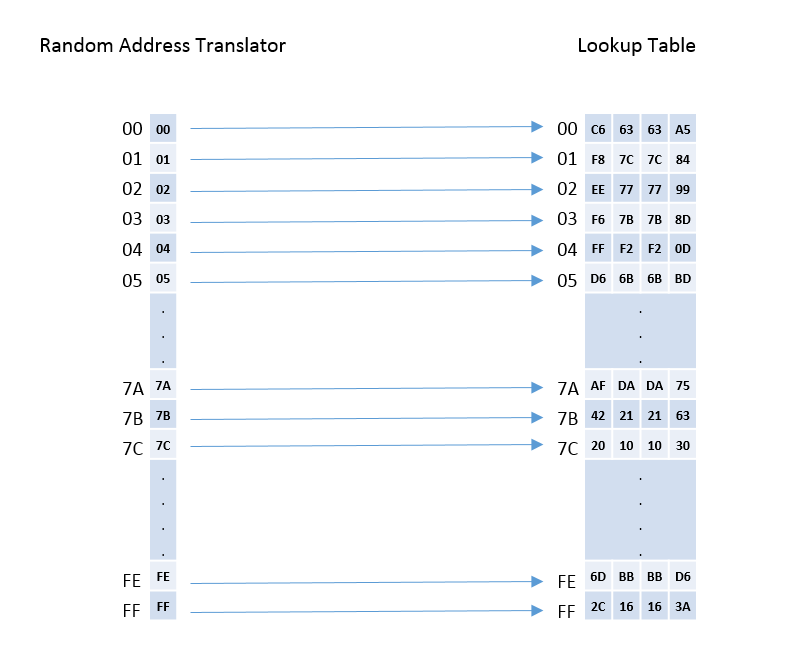
\includegraphics[scale=0.4,natwidth=785,natheight=666]{Figures/rat-init(new).png}
\captionof{figure}{Random Address Translator Initialization.}
\label{fig: Random Address Translator Initialization.}
\end{center}

The Translator table is initially aligned with the Lookup table as illustrated in figure 7. This implies that if the address of $i$-th row in the lookup table is $X_i$, the content of the $i$-th row of the Translator table is also $X_i$. So initially it has no effect on the accessed memory block of the lookup table because it is fully aligned with it. After that, lets take two rows of the Translator table $T_i$ and $T_j$ and corresponding two rows of the original lookup table $L_i$ and $L_j$ and perform a swap between them. This is illustrated in figure 8.

\begin{center}
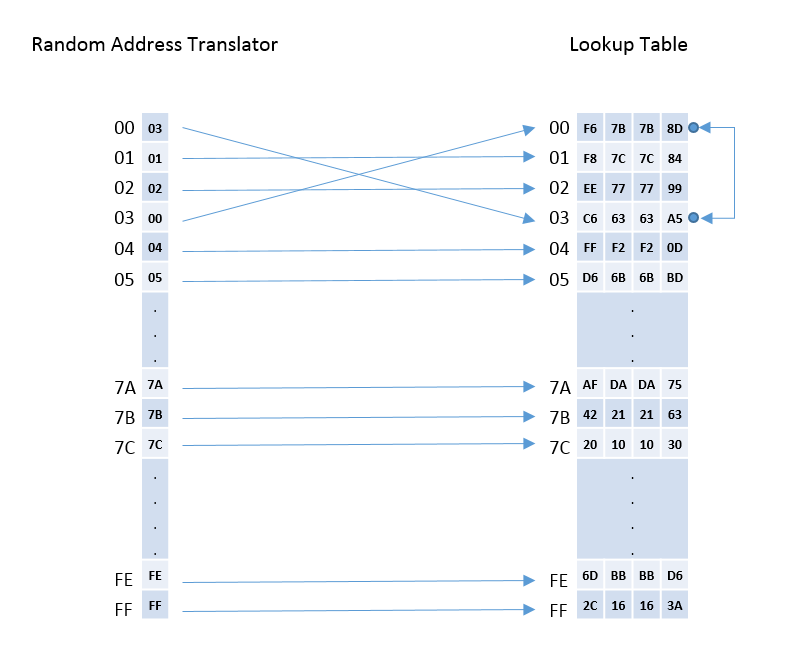
\includegraphics[scale=0.38,natwidth=785,natheight=666]{Figures/rat-step-1.png}
\captionof{figure}{Random Address Translator after first swap.}
\label{fig: Random Address Translator after first swap.}
\end{center}

Continuing this way, there can be at most 128 swaps between the entries of the table. Note that an entry can be swapped only once, so keeping trace of swapped entries is important. After scrambling, the correlation is completely broken as illustrated in figure 9.

\begin{center}
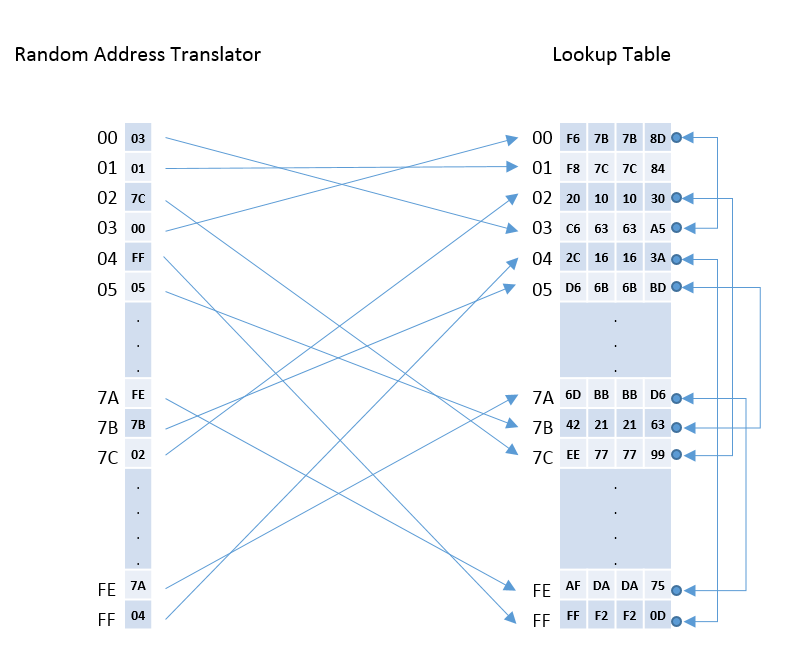
\includegraphics[scale=0.38,natwidth=785,natheight=666]{Figures/rat-scrambled(new).png}
\captionof{figure}{Random Address Translator completely scrambled. It can be noticed that some of the entries can be left ``unswapped'' as the process is arbitrary. Here 2nd entry is left intact.}
\label{fig: Random Address Translator Scrambled.}
\end{center}

With the RAT activated, there is no such phrase such as, index 0x05 will access the 1st block of the Lookup table. Because the content of the address 0x05 is now at 0x7B address (from the figure above) and that tracing is recorded by the RAT. The procedure for constructing the RAT is formulated in algorithm 2 and 3.

\begin{algorithm}
	\caption{Constructing the RAT}
	\label{Constructing the RAT}

	\begin{algorithmic}[1]
	
	\Function{init}{\null}
	\State $x\gets \{0,1,2,....,15\}$
	\State $y\gets \{0,1,2,....,15\}$
	\State $rat\gets\{0,0,0,0\}$
	\For{Arbitrary number of times}
		\State $i\gets rand() \bmod 16$\Comment{$\bmod$ resembles modulus operation}
		\State $j\gets rand() \bmod 16$
		\State $swap(x_i,x_j)$
		\State $y_{x_j}\gets i$
		\State $y_{x_i}\gets j$
	\EndFor
	\For{$i\gets0$ to $7$}
		\State $rat_0 \gets rat_0 + x_i\ll((7-i)\ll2)$\Comment{$\ll$ resemebles bitwise left shift operation}
		\State $rat_1 \gets rat_1 + x_{i+8}\ll((7-i)\ll2)$
		\State $rat_2 \gets rat_2 + y_i\ll((7-i)\ll2)$
		\State $rat_3 \gets rat_3 + y_{i+8}\ll((7-i)\ll2)$
	\EndFor
	\State delete x,y
	\State return rat
	
	\EndFunction	
	\end{algorithmic}
\end{algorithm}

After that, a scrambling is done on both tables simultaneously and arbitrarily. Note that no entry is allowed to be scrambled or swapped with other entry more than once. Also note the presence of \emph{rand()} methods. It symbolizes the randomness of the swapping process.

\begin{algorithm}
	\caption{Mapping Fuction}
	\label{Mapping Function}

	\begin{algorithmic}[1]

	\Function{map}{i}
	\If{$((i \mathrel{\&} 128)=0)$}\Comment{$\mathrel{\&}$ resembles bitwise and operation}
		\State $j \gets 0$
	\EndIf
	\State $k \gets ((255-i)\gg 4)\ll 2$\Comment{$\ll$ and $\gg$ resemble bitwise left and right shift operations respectively}
	\State $x \gets (rat_j\gg k)\mathrel{\&} 15$
	\State $y \gets i \mathrel{\&} 15$
	\State return $(x\ll 4)+y$
	\EndFunction

	\end{algorithmic}
\end{algorithm}

\begin{algorithm}
	\caption{Mingling Function}
	\label{Mingling Function}

	\begin{algorithmic}[1]

	\Function{mingle}{table}\Comment{Takes unmodified lookup table as parameter}
	\For{$i \gets 0$ to $255$}
		\For{$j \gets 0$ to $3$}
			\State $temp_{i,j} \gets table_{map(i),j}$
		\EndFor
	\EndFor
	\For{$i \gets 0$ to $255$}
		\For{$j \gets 0$ to $3$}
			\State $table_{i,j} \gets temp_{i,j}$
		\EndFor
	\EndFor
	\State delete $temp$
	\State return $table$
	\EndFunction

	\end{algorithmic}
\end{algorithm}

\begin{algorithm}
	\caption{Inverse Mapping Fuction}
	\label{Inverse Mapping Function}

	\begin{algorithmic}[1]

	\Function{inverseMap}{i}
	\State $j \gets 3$
	\If{$((i \mathrel{\&} 128)=0)$}\Comment{$\mathrel{\&}$ resembles bitwise and operation}
		\State $j \gets 2$
	\EndIf
	\State $k \gets ((255-i)\gg 4)\ll 2$\Comment{$\ll$ and $\gg$ resemble bitwise left and right shift operations respectively}
	\State $x \gets (rat_j\gg k)\mathrel{\&} 15$
	\State $y \gets i \mathrel{\&} 15$
	\State return $(x\ll 4)+y$
	\EndFunction
	\end{algorithmic}
\end{algorithm}
